\section{Dynamic branch prediction}

The main idea of dynamic branch prediction techniques is to leverage past branch behavior to forecast future outcomes.
Dynamic branch prediction integrates two key mechanisms:
\begin{itemize}
    \item \textit{Branch outcome predictor}: determines the likelihood of branch direction based on historical behavior.
    \item \textit{Branch target predictor}: forecasts the target address for a taken branch.
\end{itemize}
These prediction modules collaborate within the instruction fetch unit, aiding in the prediction of the subsequent instruction to fetch from the instruction cache:
if the branch isn't taken, the PC increments; otherwise the BTP provides the target address.

\subsection{Branch History Table}
The Branch History Table (BHT) is a data structure where each entry consists of a single bit, representing whether a branch was recently taken or not. 
This table is pivotal in branch prediction mechanisms.

The BHT operates by predicting the outcome of branches based on recent history:
\begin{itemize}
    \item \textit{Initial prediction}: when encountering a branch, the BHT provides a prediction based on its stored history. 
        If the history indicates that the branch has been frequently taken, the BHT predicts that the branch will be taken again.
    \item \textit{Execution flow}: the processor begins fetching instructions in the predicted direction, assuming the correctness of the prediction.
    \item \textit{Validation}: if the prediction proves correct, execution proceeds smoothly.
        However, if the branch prediction is incorrect the prediction bit associated with that branch in the BHT is updated to reflect the correct outcome.
        Then, the pipeline is flushed to discard any instructions fetched based on the incorrect prediction and the correct instructions are then fetched and executed based on the accurate branch outcome.
\end{itemize}
\begin{figure}[H]
    \centering
    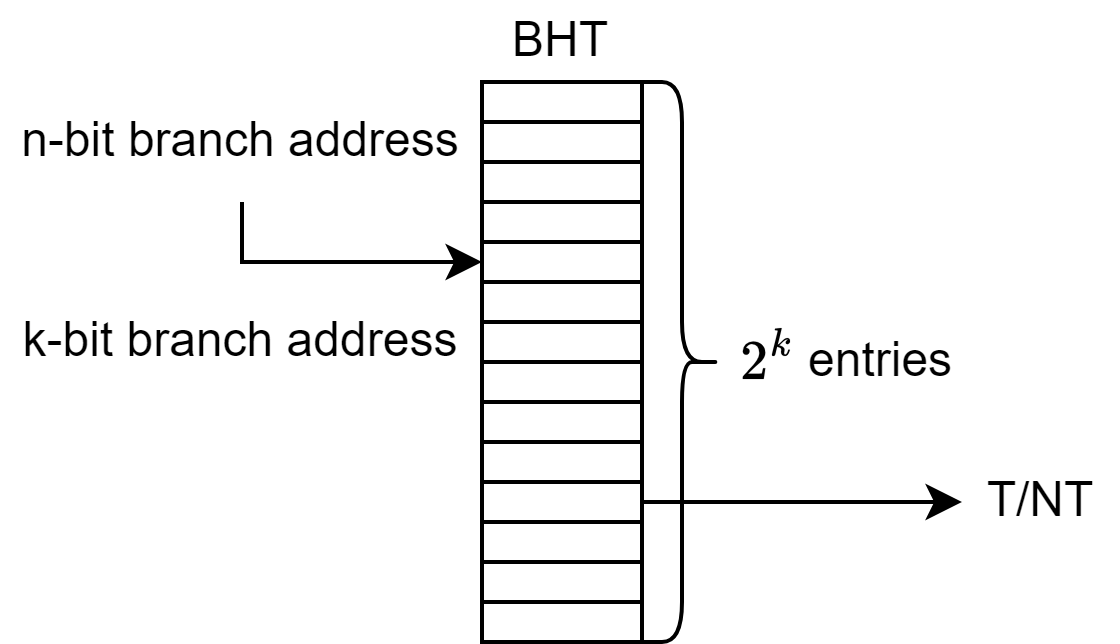
\includegraphics[width=0.5\linewidth]{images/bht.png}
    \caption{BHT structure}
\end{figure}
Mispredictions can occur due to: incorrect predictions for specific branches, or conflicting history at the same index when multiple branches reference it, leading to inaccurate predictions.
To mitigate mispredictions:
\begin{itemize}
    \item \textit{Increase BHT size}: by expanding the number of rows in the BHT, more branches can be tracked simultaneously, reducing the likelihood of conflicting histories.
    \item \textit{Hashing function}: employing a hashing function for indexing can distribute branches more evenly across the BHT, minimizing index collisions and improving prediction accuracy.
\end{itemize}

\paragraph*{One bit BHT}
The 1-bit BHT has a notable limitation, especially evident in loop branches. 
Even if a branch is mostly taken throughout a loop but is not taken once, the 1-bit BHT may mispredict twice instead of once. 
This results in two erroneous predictions:
\begin{itemize}
    \item At the end of the loop iteration, where the prediction bit suggests a taken branch, contradicting the need to exit the loop.
    \item When re-entering the loop after the first iteration's end, the prediction bit indicates an exit from the loop, stemming from the final iteration's flipped prediction bit.
\end{itemize}

\paragraph*{Two bit BHT}
In contrast, the 2-bit BHT requires two consecutive prediction failures before altering its prediction. 
For a loop branch, during the final iteration, there is no need to change the prediction.
 Each index in the table employs 2 bits, encoding the four states of a finite state machine.

\paragraph*{Higher bit BHT}
In the case of an $n$-bit BHT, each entry in the prediction buffer requires an $n$-bit saturating counter. 
This counter ranges from $0$ to $2^n-1$.
If the counter equals or exceeds half of its maximum value, the branch is predicted as taken; otherwise, as untaken.
Similar to the 2-bit scheme, a taken branch increments the counter, while an untaken branch decrements it. 
Research suggests that 2-bit predictors perform nearly as effectively as higher bit predictors.

\subsection{Branch target predictor}
The Branch Target Buffer (BTB), also referred to as a branch target predictor, acts as a cache that stores the predicted target address for instructions following a branch.
During the IF stage, the BTB is accessed using the instruction address of the fetched instruction, which may include a branch, to index the cache.
Typical entries in the BTB include the exact address of a branch, and the predicted target address.
\begin{figure}[H]
    \centering
    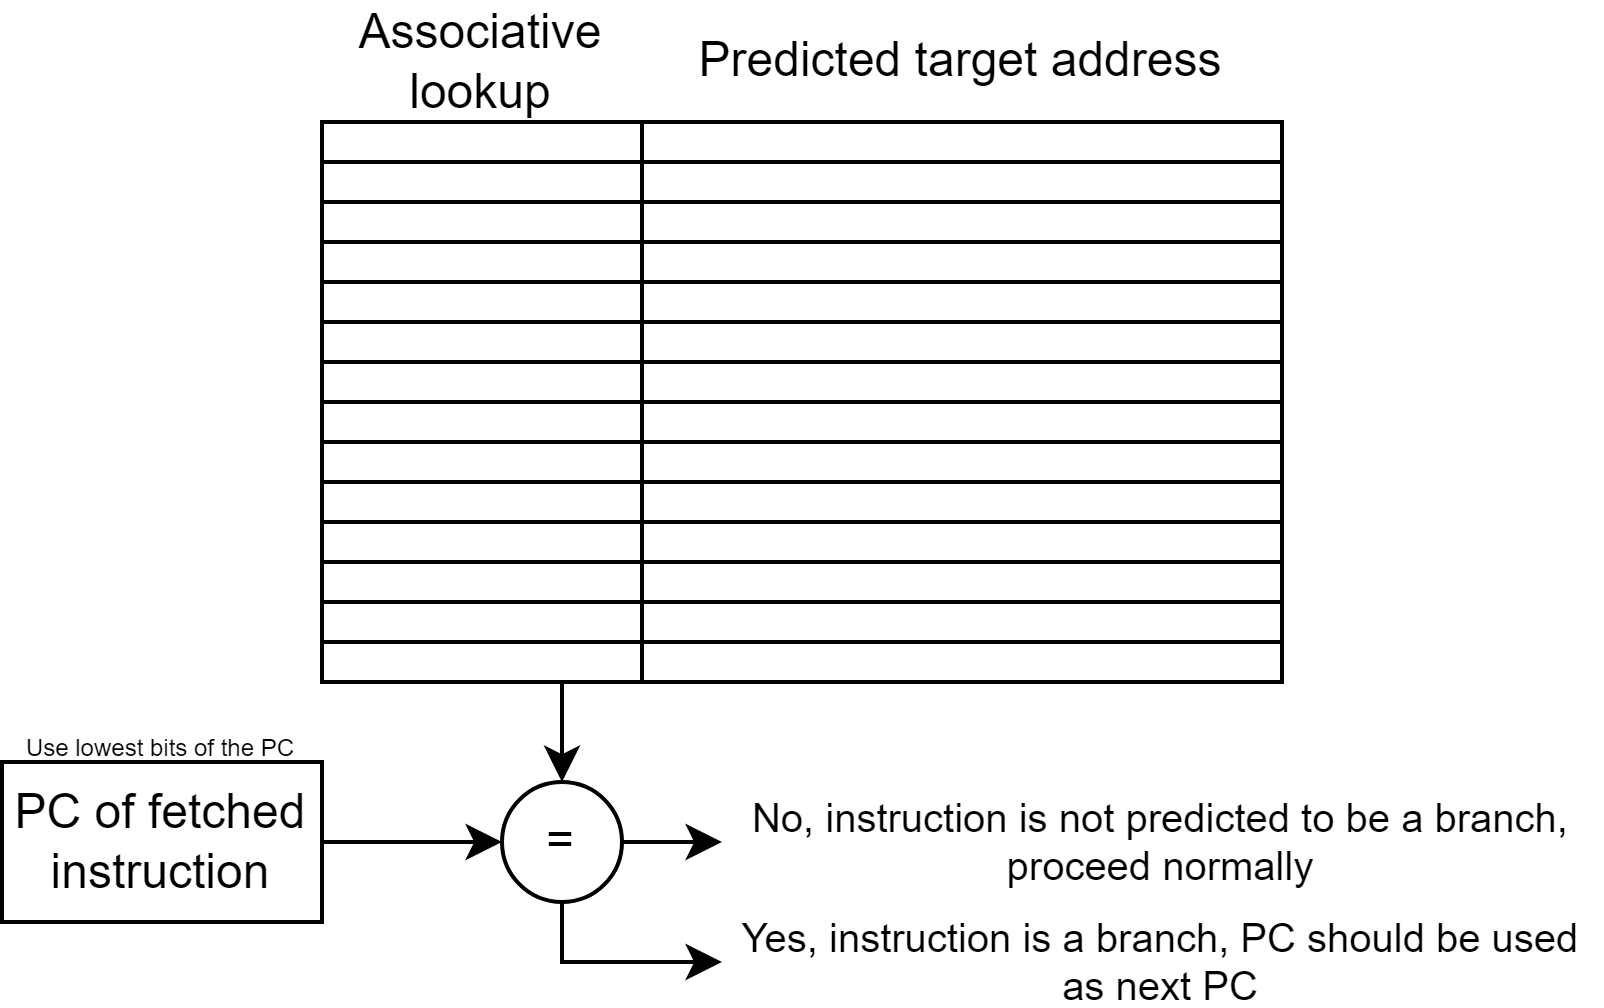
\includegraphics[width=0.5\linewidth]{images/btb.png}
    \caption{Branch target buffer structure}
\end{figure}

\subsection{Correlating branch predictors}
BHT predictors rely solely on the recent behavior of a single branch to forecast its future behavior.
Correlating branch predictors, however, operate on the principle that recent branches exhibit correlations. 
This means that not only the current branch under consideration but also other recent branches can influence the prediction of the current branch.
Predictors that utilize the behavior of other branches to make predictions are known as correlating predictors or 2-level predictors.

In a general ($m, n$) correlating predictor, the system maintains a history of the last $m$ branches to select from $2^m$ BHTs, each being an $n$-bit predictor.

\paragraph*{Accuracy}
A 2-bit predictor without global history can be seen as a ($0, 2$) predictor.
Comparing the performance of a simple 2-bit predictor to a ($2, 2$) correlating predictor it often outperforms a 2-bit predictor regardless of the number of entries.

\paragraph*{Two-level adaptive branch predictors}
In two-level adaptive branch predictors:
\begin{itemize}
    \item The first-level history is stored in one or more k-bit shift registers called the Branch History Register (BHR), which records outcomes of the k most recent branches.
    \item The second-level history is stored in one or more tables known as the Pattern History Table (PHT), consisting of two-bit saturating counters.
\end{itemize}
The BHR is used to index the PHT to determine which 2-bit counter to use for prediction.
Several types of two-level predictors include: BHT (local), GAs (global), and GShare (combination of local and global).